%----------------------------------------------------------------------------
\chapter{Mérési eredmények}
%----------------------------------------------------------------------------

Ebben a fejezetben a teljesítménymérések eredményének elemzéséről és a leszűrhető konklúziókról lesz szó. Összehasonlítjuk a Graph Engine teljesítményét a másik két eszköz teljesítményével. Kielemezzük a lehetséges okait a futási idők közötti különbségeknek.

\section{Mérés és az eredmények elmentése}

Minden szakasz futási ideje a \emph{System.Diagnostic.StopWatch} osztály segítségével lett lemérve. A többi Train Benchmark implementáció $ns$-ban ad eredményt a futás idejéről, azonban két azonos konfigurációjú , egymás után történő futtatás eredménye is legalább 100 $\mu{}s$-mal eltér. Ezen megfontolás miatt az elkészült program futásidő-mérésének pontossága 1 $\mu{}$s. A \emph{StopWatch} osztályban az \texttt{ElapsedTicks} és a \texttt{Frequency} \emph{property}-k segítségével lehet $ms$-nál pontosabb eredményt elérni.

A méréseket ötször egymás után hajtja végre a program és az eredményt egy \emph{csv} fájlba fűzi bele. Az öt egymás utáni futtatás nagyobb valószínűséggel ad konzisztens eredményt. A \emph{csv} minden sorába egy adott futtatás szakaszának (beolvasás, ellenőrzés, módosítás vagy újraellenőrzés) az eredménye kerül. A felépítése az alábbi oszlopokból áll:

\begin{itemize}
	\item \emph{Tool}: Annak az adatbázis-rendszernek a neve, amin a programot futtatjuk.
	\item \emph{Workload}: \emph{Inject} vagy \emph{Repair} lehet, az alapján hogy milyen teljesítményt mérünk, a hibainjektálást vagy a javítást.
	\item \emph{Description}: Leírást illeszthetünk ide. Ez az elkészült szoftver futtatása után üres lesz.
	\item \emph{Model}: A modell neve és mérete kerül ide.
	\item \emph{Run}: Aktuális futtatás sorszáma 1-től indexelve.
	\item \emph{Phase}: A futtatott szakasz típusa kerül ide, értéke \emph{Read}, \emph{Check}, \emph{Transformation} vagy \emph{Recheck} lehet.
	\item \emph{Iteration}: A módosítás és újraellenőrzés szakasz többszörös futtatásának sorszáma. A beolvasás- és a validációs szakaszban nincsen értéke.
	\item \emph{Time}: Az adott szakasz futtatása alatt eltelt idő $ns$-ban. Nem a teljesítménymérés kezdete óta eltelt időt jelzi.
\end{itemize}

A gép konfigurációja, melyen a méréseket végeztük a \ref{tab:System} táblázatban található. A meghajtón több, mint 20 GB szabad hely volt elérhető.

\begin{table}[H]
	\centering
	\begin{TAB}(r,20pt,20pt){|c|c|}{|c|c|c|c|c|} 
		Alaplap & Gigabyte Z87M-D3H \\
		Processzor & Intel\textregistered{} Core\texttrademark{} i5-4690K CPU @ 3.50GHz \\ 
		Memória & Kingston 8GB 1600MHz DDR3 Non-ECC CL11 \\
		Meghajtó & Kingston HyperX 3K 240 GB SSD  \\
		Operációs rendszer & Windows 7 Ultimate x64 Service Pack 1  \\ 
	\end{TAB}
	\caption{A gép konfigurációja}
	\label{tab:System}
\end{table}

Az elkészült program és a Train Benchmark többi teljesítménymérésének futtatása sok órás művelet. A modellek (amiken a teszteket végeztük) elemeinek a száma körülbelül 5 ezertől 9,3 millióig terjed kettes alapú logaritmikus skálán. Olyan esetben, amikor egy eszköz egy szakaszban lévő futási ideje túllépne egy bizonyos észszerű határt, akkor leállítjuk a teljesítménymérést. Ezt a határt a \emph{RouteSensor} esetében 100000 $ms$-nál, a \emph{SwitchSet} kényszer esetében 200000 $ms$-nál húztuk meg. Amennyiben bármelyik szakaszban (beolvasás, ellenőrzés vagy módosítás) a futási idő meghaladja ezt a határt, akkor értelemszerűen a többi szakaszban sem kapunk eredményt.

A tesztek eredményét a következő részeken keresztül mutatjuk be. Az első két példa a modell beolvasása után a \emph{RouteSensor} kényszer teljesülését ellenőrzi, majd az ahhoz kapcsolódó \emph{Inject}, illetve \emph{Repair} transzformációt hajtja végre. A második két példa a \emph{SwitchSet} kényszert követeli meg. Minden esetben, a modelleken ötször futtattuk le a teljes ciklust és azon belül a módosítás, újraellenőrzés fázisokat tizenháromszor, végül pedig az egész átlagából számoltuk ki az idő értékeket.

Minden eszköz tesztjét egy parancssori ablakból futtattuk, ezáltal törekedve arra, hogy más programok ne használják a számítógép erőforrásait. A tesztek után az eredmények kiértékelése céljából lefuttattuk úgy is, hogy közben a \emph{Visual Studio} beépített teljesítményanalízisével mértük, hogy melyik függvény végrehajtása tart a legtovább.

\section{A \emph{RouteSensor}-hoz tartozó \emph{Inject} eredményeinek értékelése}

A \ref{fig:RouteSensorInjectResult} ábra mutatja 6 diagramon a tesztelés eredményét. A diagramokon a függőleges tengely a futási idő $ms$-ban mért logaritmikus skáláját, míg a vízszintes tengely a modellek méretének skáláját mutatja. Ez utóbbi is logaritmikus skála, mert egy osztás alatt a modellek mérete duplájára növekszik. A diagramok tetején található felirat az adott futtatási fázist mutatják.

A továbbiakban egyesével a diagramokon látható eredményeket elemezzük. Az átláthatóság érdekében a vízszintesen egymás mellett elhelyezkedő diagramok skálája megegyezik.

\subsubsection{Read}

A \emph{Read} szakaszban a Graph Engine minden modell esetében az adatok beolvasása és feldolgozása több ideig tartott. Ennek oka az, hogy az \emph{RDF} formátum feldolgozását és memóriába másolását a használt könyvtár (\emph{dotNetRDF}) időigényesen végezte.

\subsubsection{Check}

A validációs szakasz során a kapott eredmények alapján a Graph Engine futási idejét lényegesen nem befolyásolta a modell mérete. Ennek valószínűsíthető oka, hogy az adatbázis felé indított kérés feldolgozási ideje lassú, de a kérést már gyorsan dolgozza fel, az adatok mennyiségétől függetlenül.

\subsubsection{Read and Check}

A \emph{Read and Check} diagram az előző kettő összegét mutatja. A beolvasási szakasz több nagyságrenddel nagyobb a validációsnál, így az a meghatározó. A Graph Engine hiába gyorsabb nagy modelleknél a validációs szakaszban, ez az előny az összesített időknél eltűnik. 

\pagebreak
\begin{figure}[H]
	\centering
	\vspace*{-2cm}
	\makebox[\linewidth]{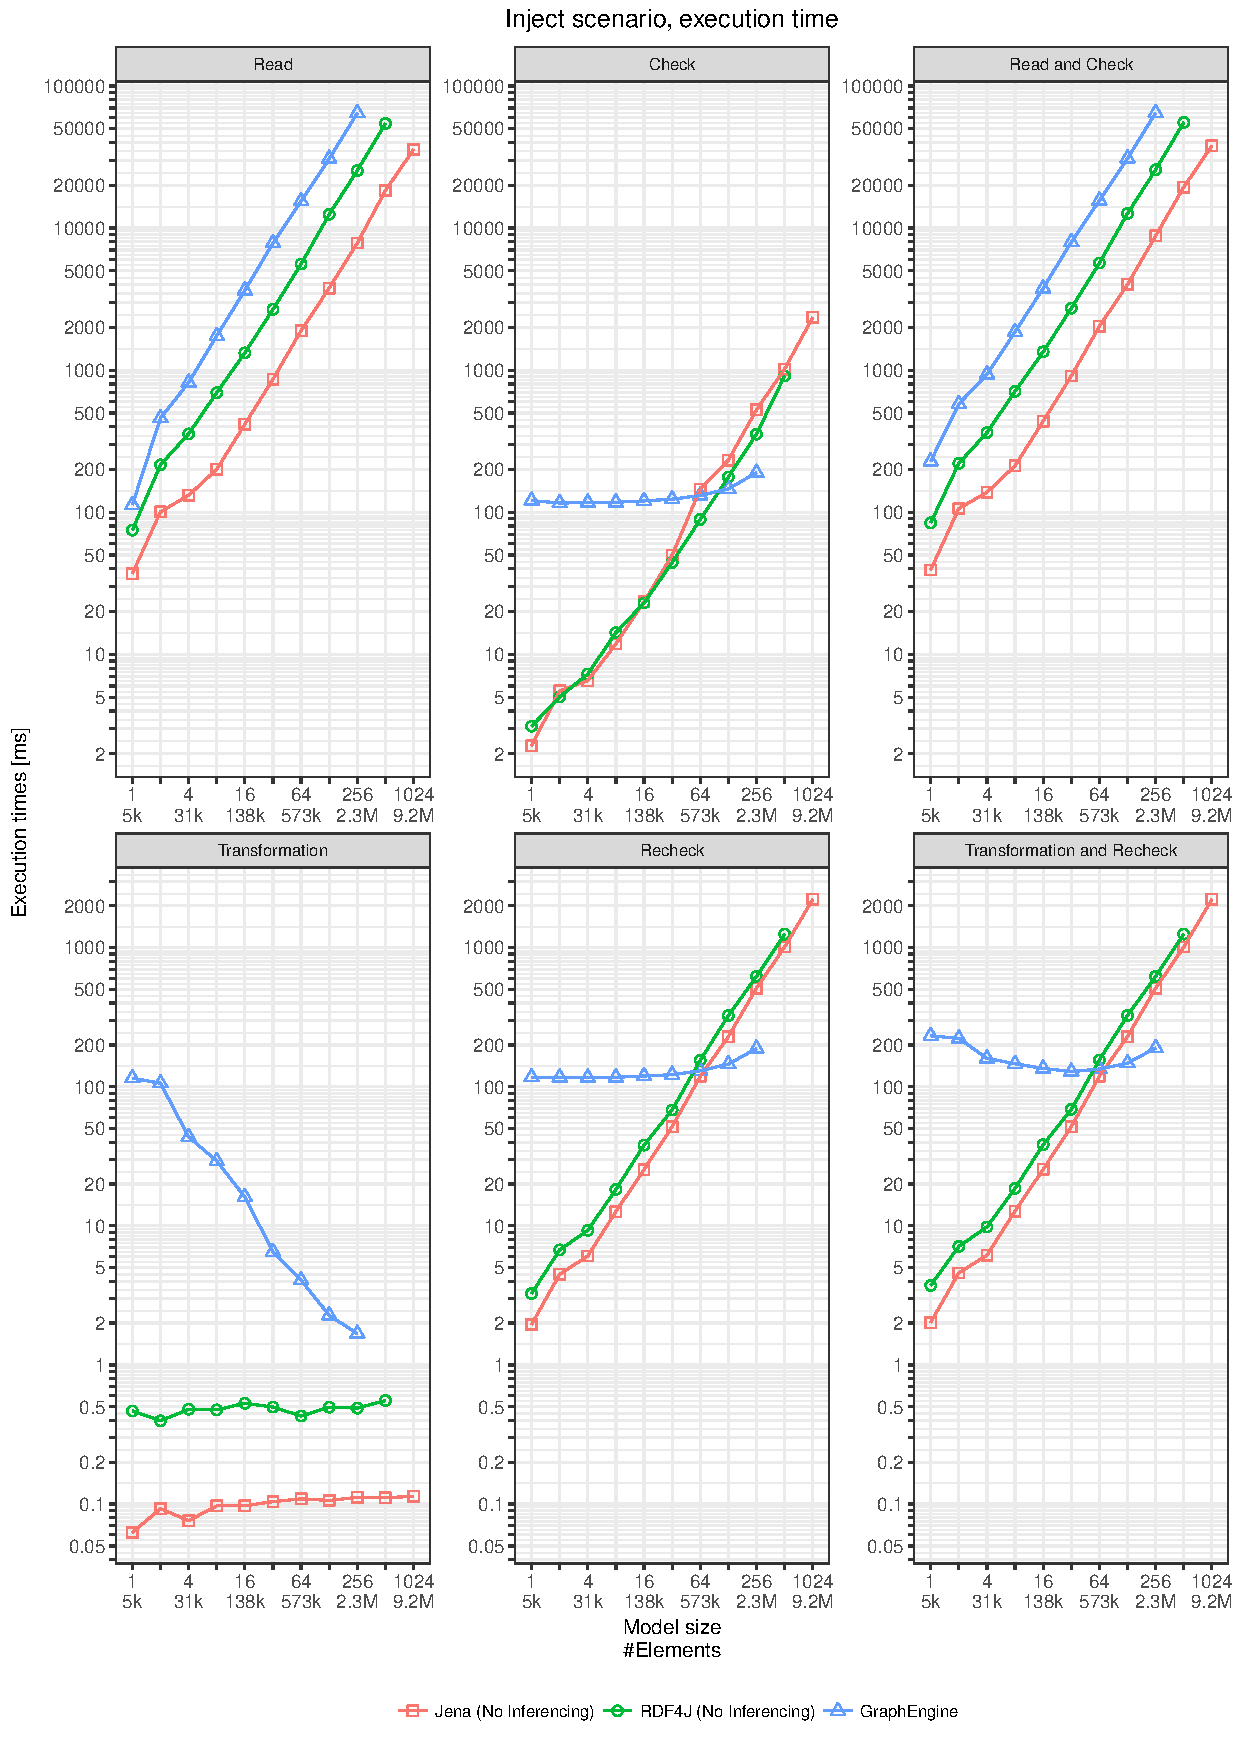
\includegraphics[width=1\linewidth]{figures/RouteSensor-times-Inject.pdf}}
	\caption{A hibainjektálás tesztelésének futási idejeinek eredménye a \emph{RouteSensor} esetében.}
	\label{fig:RouteSensorInjectResult}
\end{figure}

\subsubsection{Transformation}

A hibainjektálás során előre nem várt eredményt kaptunk. A modell növekedésével a Graph Engine teljesítménye nőtt, a futási idő rövidebb lett. Ennek oka, hogy kisméretű modelleken több lekérdezés kellett, hogy találjon olyan \emph{requires} élt, amit el lehet távolítani. Az \emph{RDF4J} és a \emph{Jena} esetében a modell mérete nem befolyásolta az eredményt. A \emph{Read} szakasz lassú futása miatt a legnagyobb méretű modelleken nem volt tesztelhető, hogy meddig csökkenne tovább.

\subsubsection{Recheck}

A \emph{Recheck} fázisban a \emph{Check} szakasszal megegyező eredményt kaptunk az összes eszköznél. Ennek oka, hogy nem tárolunk információt arról, hogy az előző validációs fázisban milyen eredményre jutottunk, ezáltal az újraellenőrzésnél ismét a teljes modellt be kell járni. Gyorsítható lenne a folyamat, ha eltárolnánk, hogy az előző ellenőrzés hol talált olyan csúcsokat, melyek nem feleltek meg a kényszernek és az újraellenőrzésnél a modell többi részében keresne csak hibákat. Azonban ehhez feltételezni kell, hogy ismerjük a szimuláció működését, azaz a transzformációs fázisban nem javítunk ki hibákat.

\subsubsection{Transformation and Recheck}

Hasonlóan a \emph{Read and Check} diagramon látható eredményhez, itt is az egyik fázis sokkal több idő alatt fut le, ezáltal az együttes eredményben dominál. Itt azonban a validációs fázis a meghatározó. Kis modellek esetén ugyan befolyásolja a Graph Engine eredményét, de nagyobb méretű modelleken nem.

\section{A \emph{RouteSensor}-hoz tartozó \emph{Repair} eredményeinek értékelése}

A \emph{Repair} tesztelés esetében a beolvasás és a validáció ugyanolyan eredményt adott, mint az \emph{Inject} esetében. Ez a várt eredmény, hiszen ugyanazok a függvények futottak le. Így csak a módosítás fázisban van eltérés.

A \ref{fig:RouteSensorRepairResultTransformation} ábrán a \emph{Transformation} és a \emph{Transformation and Recheck} fázisok futásidejei találhatóak. A várakozásnak megfelelően a Graph Engine módosítás fázisban töltött ideje a tesztelt modellekre nem csökkent, de nem is nőtt számottevően. A másik két eszköz esetében exponenciálisan növekedett a végrehajtási idő. Az \emph{RDF4J} és a \emph{Jena} esetében nem csak az \emph{Inject}, de a \emph{Repair} módosításnál is a modell ellenőrzése minden mért eredménynél több, mint tízszer annyi, így a \emph{Transformation and Recheck} szakasz idejét a \emph{Transformation} csak kis mértékben befolyásolja. Ezzel szemben a Graph Engine esetében a módosítás és az újraellenőrzés fázisok időben nagyságrendileg megegyeznek, így a kettő egyforma mértékben befolyásolja az eredményt.

\begin{figure}[H]
	\centering
	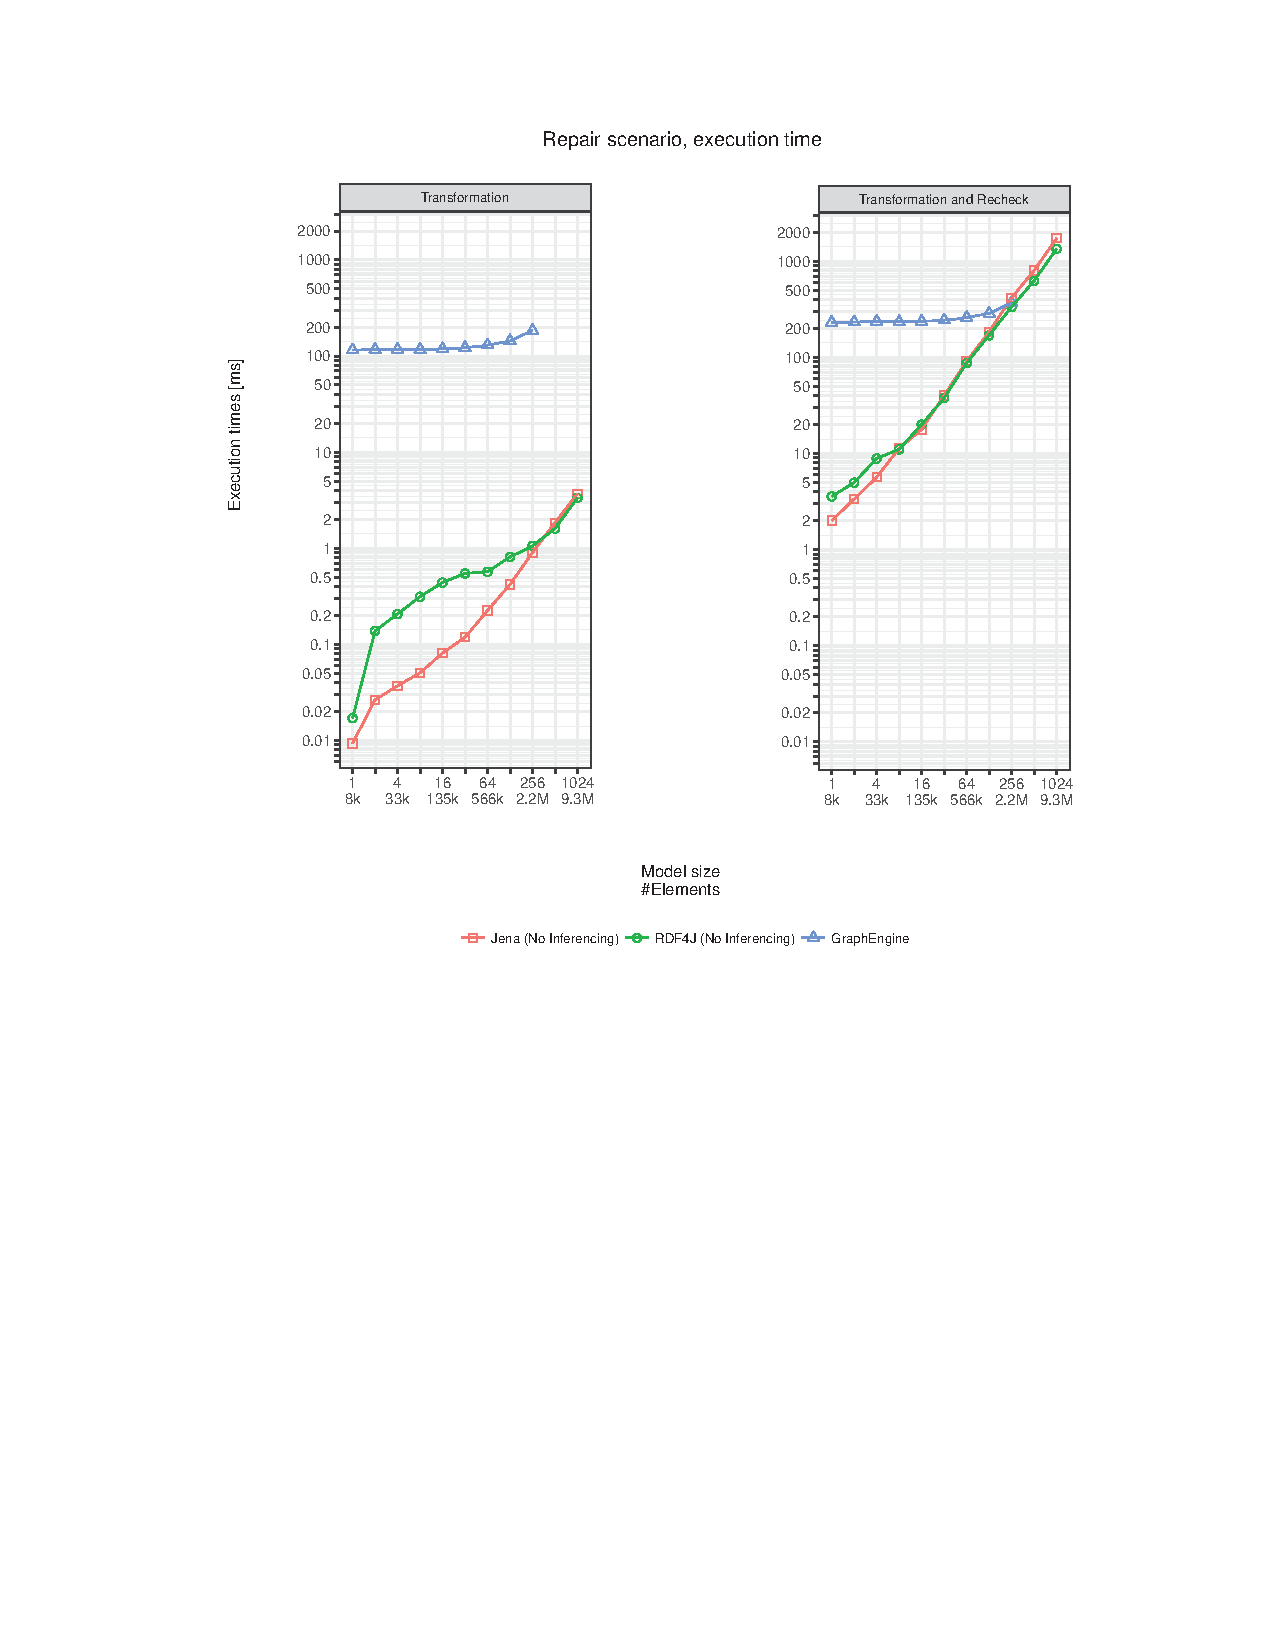
\includegraphics{figures/RouteSensor-times-Repair-Transformation-Recheck.pdf}
	\caption{A modelljavítás tesztelésének eredménye a \emph{RouteSensor} kényszer esetében.}
	\label{fig:RouteSensorRepairResultTransformation}
\end{figure}

%\section{A \emph{SwitchSet}-hez tartozó \emph{Inject} eredményeinek értékelése}
%
%A továbbiakban a \emph{SwitchSet} kényszer teljesülésének a feltételét vizsgáltuk. A modellbe a hibainjektálás és a javítás is a \emph{SwitchSet} kényszernek megfelelően történt. Az eredmények diagramja a \ref{fig:SwitchSetInjectResult} ábrán látható.
%
%A \emph{Read} fázisban a várakozásunknak megfelelően nem változott a teljesítmény. Azonban a \emph{RouteSensor}-hoz képest itt a Graph Engine csak eggyel kisebb modell esetében futott le elfogadható időn belül, az \emph{RDF4J} pedig eggyel nagyobbnál is.
%
%\pagebreak
%\begin{figure}[H]
%	\centering
%	\vspace*{-2cm}
%	\makebox[\linewidth]{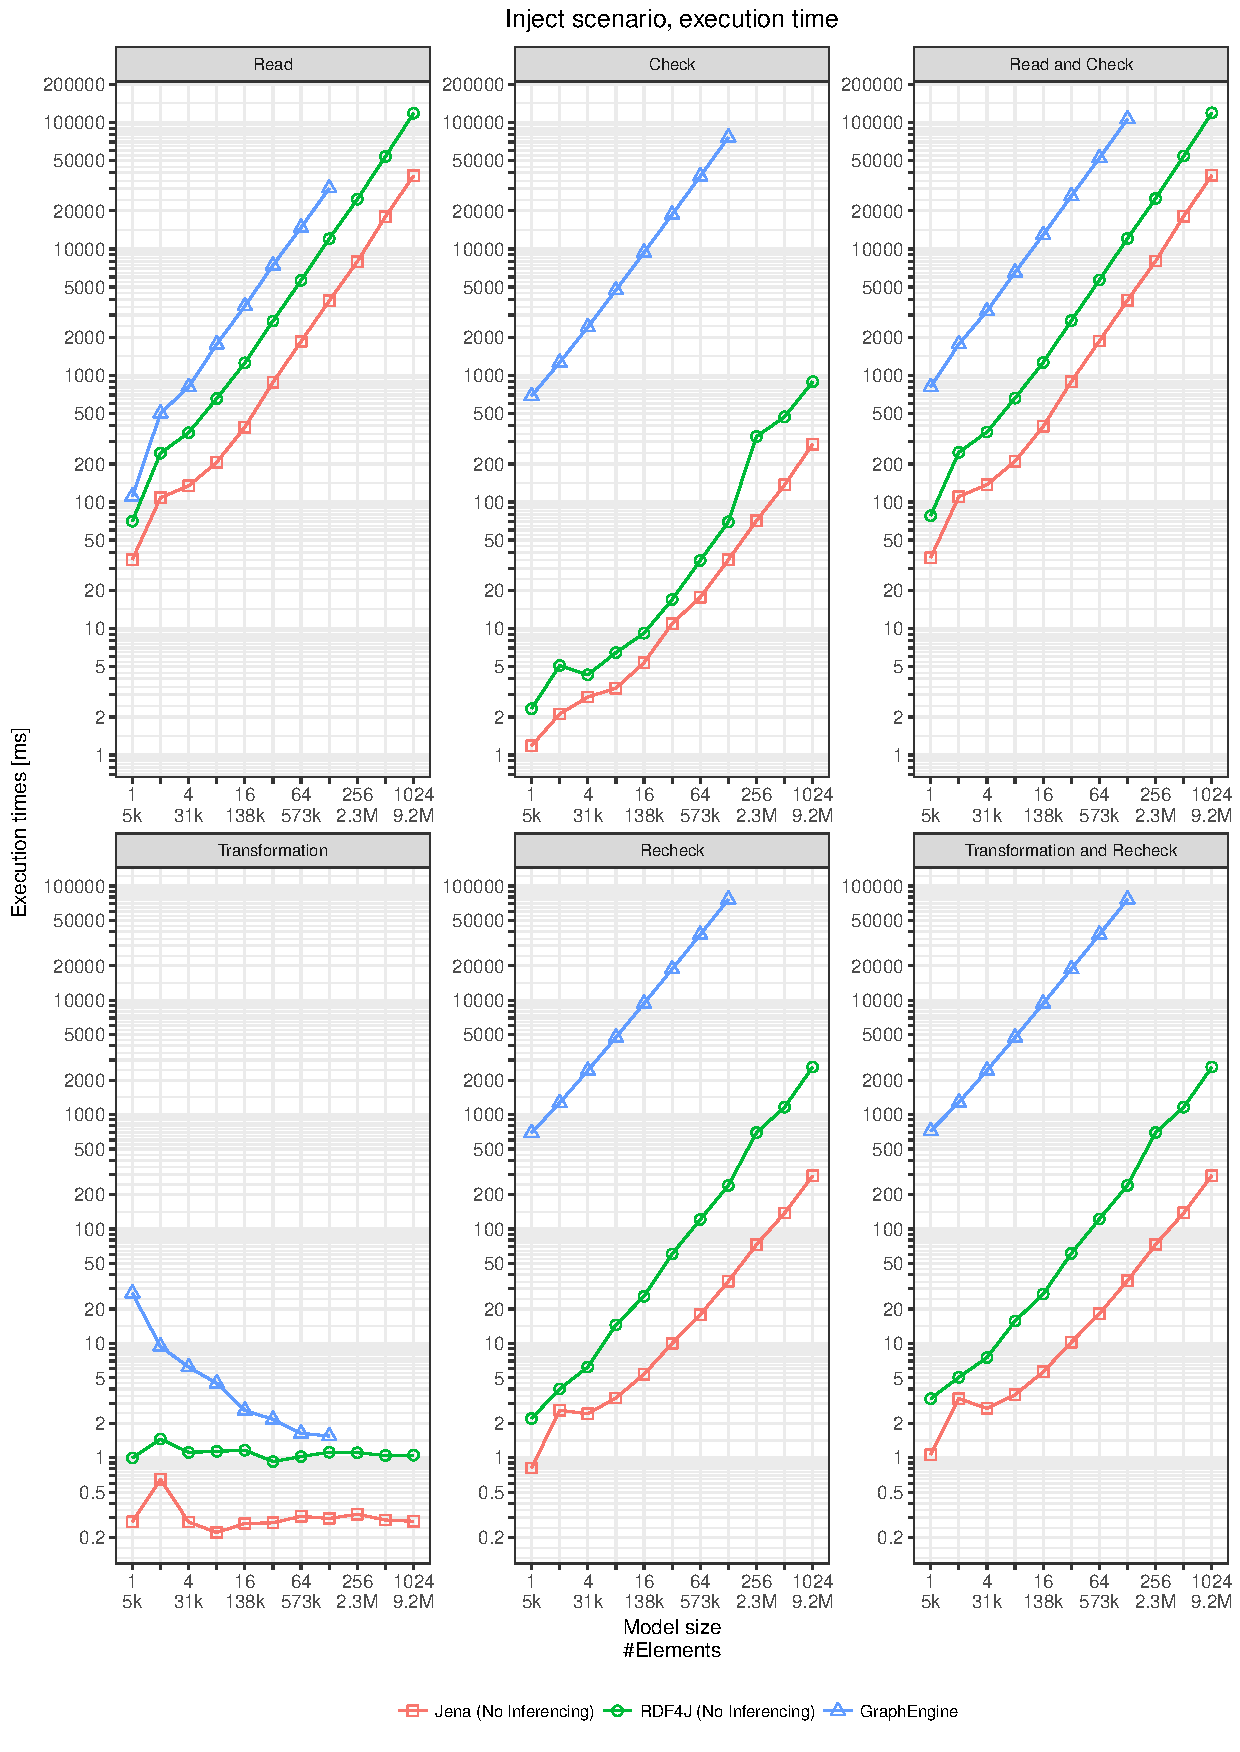
\includegraphics[width=1\linewidth]{figures/SwitchSet-times-Inject.pdf}}
%	\caption{A hibainjektálás tesztelésének futási idejeinek eredménye a \emph{SwitchSet} esetében.}
%	\label{fig:SwitchSetInjectResult}
%\end{figure}
%
%\subsubsection{Check és Recheck}
%
%A validációs fázisokban szemmel láthatóan elmarad a Graph Engine teljesítménye a többi eszközéhez képest. A futási idő bizonyos modelleknél több, mint 1000-szerese a másik két eszközének. Emellett a \emph{Jena} és az \emph{RDF4J} teljesítménye nőtt a \emph{RouteSensor} kényszer validációs teljesítményméréséhez képest, azonban a Graph Engine-é jelentős mértékben csökkent.
%
%Ennek az oka, hogy a \emph{SwitchSet} kényszerhez két \emph{LINQ} lekérdezés, ezáltal három \emph{foreach} ciklus van egymásba ágyazva, míg a \emph{RouteSensor}-nál csak egy \emph{LINQ} lekérdezés van. Az, hogy minden lekérdezés után az összes adatot el kell menteni a kliensoldali memóriába, emellett az adatbázishoz is rengeteg lekérdezést kell intézni a validációhoz, ezt az eredményt produkálta. Sokat javítana a teljesítményen, ha az adatbázishoz csak egy kérést kellene küldeni, azonban ez egyelőre nem megoldható, ugyanis több típusú gráfcsúcsot kell lekérdezni a kényszer validációjához.
%
%\subsubsection{Read and Check}
%
%A \emph{RouteSensor} kényszerhez tartozó \emph{Inject} méréssel ellentétben a \emph{Read and Check} szakaszban a validáció ideje a számottevőbb.
%
%\subsubsection{Transformation}
%
%A módosítás fázisban az \emph{RDF4J} és a \emph{Jena} teljesítménye kis kilengésekkel, konstans értéken marad a futási idő szempontjából. A Graph Engine esetében, hasonlóan a \emph{RouteSensor} módosításhoz képest, nagyobb modellekre rövidebb időértékeket mértünk, mint kisebbekre.
%
%\section{A \emph{SwitchSet}-hez tartozó \emph{Repair} eredményeinek értékelése}
%
%A \emph{SwitchSet} kényszer validációs teljesítménymérésének eredménye a beolvasás és validációs fázisokban megegyezik a hibainjektálásnál kapott eredményekkel. A módosítás fázisban a validációs szakasszal megegyező eredményt kaptunk. A módosításhoz először megkeresi azt, hogy hol található hiba, aztán kijavítja. Azonban azt megkeresni

\section{\emph{Performance Profiler}}

A \emph{Visual Studio} beépített \emph{Performance Profiler} funkciójával elemezni lehet egy \emph{.NET} platformon futó programot. Ezt arra használtuk, hogy megállapítsuk melyik az a függvényhívás, ahol a program a legtöbb időt tölti. Emellett lehetőség van azt is vizsgálni, hogy egy függvény hányszor hívódott meg. A \emph{Profiler} eredménye azt mutatta, hogy a \texttt{System.Collections.IEnumerator.MoveNext()} függvény végrehajtásával tölti a legtöbb időt a processzor. Ez egy \emph{LINQ} lekérdezés után az eredményeken való végigiterálásnál hívódik. Második helyen az \emph{TurtleParser} \texttt{Load()} metódusa áll, ami a \emph{dotNetRDF} könyvtár beolvasásért felelős függvénye.

%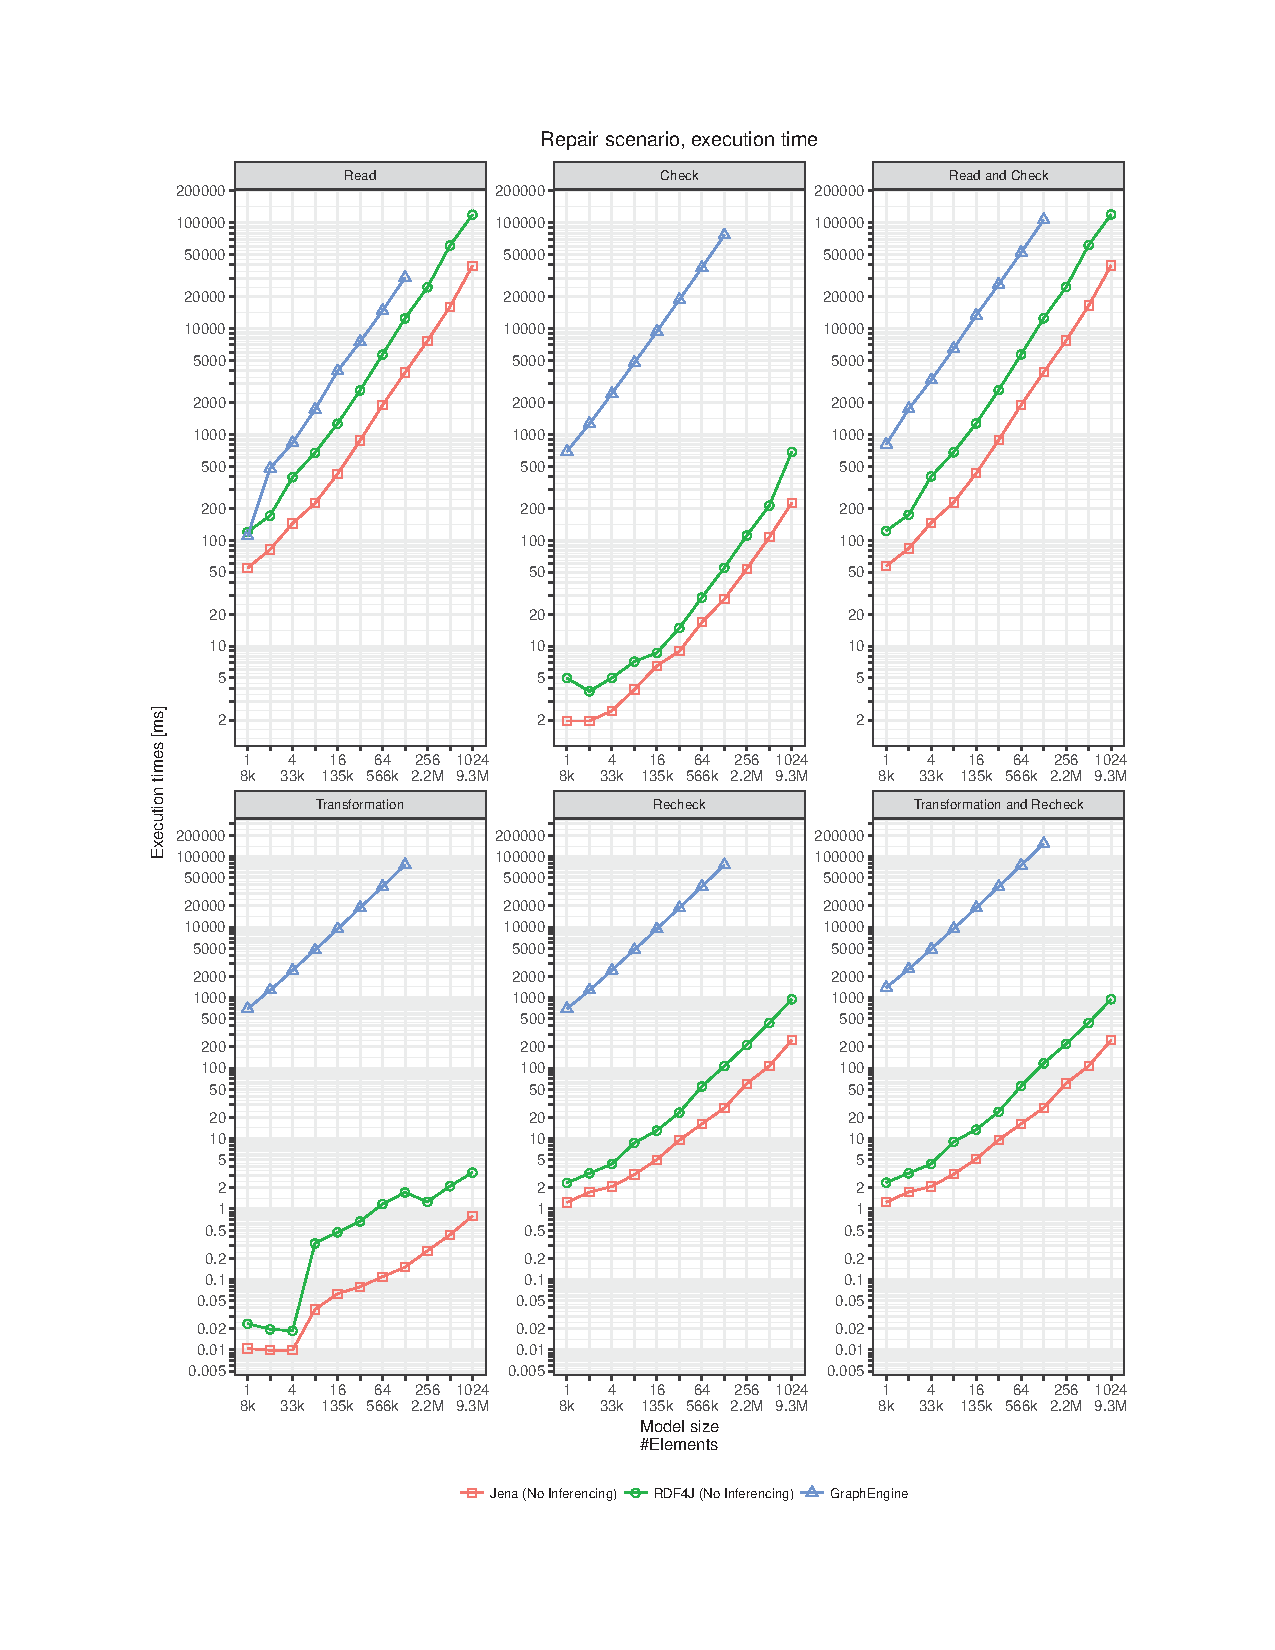
\includepdf[pagecommand={}]{figures/times-Repair.pdf}